\item \textbf{{[}PJC/PRELIM/9597/2017/P1/Q2{]} }

A circular queue is to be implemented with a fixed size array of n
elements, indexed from \texttt{0} to \texttt{(n \textendash{} 1)}.
\begin{center}
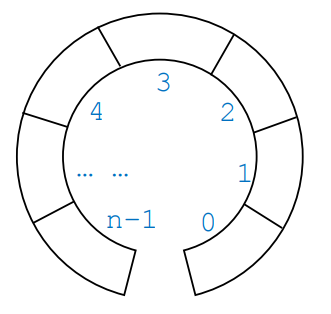
\includegraphics[width=0.2\paperwidth]{C:/Users/Admin/Desktop/Github/question_bank/LyX/static/img/9597-PJC-2017-P1-Q2-1}
\par\end{center}

\subsection*{Task 2.1 }

Following good programming practice, write program code for procedures 
\begin{itemize}
\item \texttt{setup\_queue} to set up circular queue which allows user to
input the value of \texttt{n}, 
\item \texttt{enqueue} to add an element to the queue,
\item \texttt{dequeue} to remove an element from the queue. 
\end{itemize}

\subsection*{Evidence 5: }

Program code for Task 2.1 for \texttt{setup\_queue}, \texttt{enqueue},
\texttt{dequeue}. \hfill{}{[}12{]}

\subsection*{Task 2.2 }

Write program code for a main procedure to display a menu with these
options: 
\noindent \begin{center}
\begin{tabular}{|l|}
\hline 
\texttt{1. Set up queue}\tabularnewline
\texttt{2. Add to queue}\tabularnewline
\texttt{3. Remove from queue}\tabularnewline
\texttt{4. Display queue }\tabularnewline
\texttt{5. Exit}\tabularnewline
\hline 
\end{tabular}
\par\end{center}

Write additional code to implement menu options 1, 2 and 3 using procedures
from Task 2.1. 

Also write code to implement 
\begin{itemize}
\item option 4 to display the contents of the queue and its pointers as
shown in diagram below, 
\item option 5 to exit program. 
\end{itemize}
The diagram shows the result of option 4 to display contents of queue
and pointers for \texttt{n=5} with 3 items \texttt{'fig'}, \texttt{'lemon'}
and \texttt{'cane'} in the queue:
\noindent \begin{center}
\begin{tabular}{l|l|l}
\multicolumn{1}{l}{} & \multicolumn{1}{l}{\texttt{Queue}} & \tabularnewline
 & \texttt{fig} & \texttt{<- Front pointer}\tabularnewline
 & \texttt{lemon} & \tabularnewline
 & \texttt{cane} & \texttt{<- Rear pointer}\tabularnewline
 &  & \tabularnewline
 &  & \tabularnewline
\multicolumn{1}{l}{} & \multicolumn{1}{l}{} & \tabularnewline
\multicolumn{1}{l}{} & \multicolumn{2}{l}{\texttt{Number in queue: 3}}\tabularnewline
\end{tabular}
\par\end{center}


\subsection*{Evidence 6:}

Program code for Task 2.2 for main procedure, display queue and exit
program. \hfill{}{[}8{]}

\subsection*{Task 2.3 }

Test run your program from using the following input: 
\noindent \begin{center}
\begin{tabular}{|l|}
\hline 
\texttt{Test run 1}\tabularnewline
\hline 
- \texttt{n = 8}\tabularnewline
- Add 5 words to queue in order:\tabularnewline
\texttt{'Mary', 'had', 'a', 'little', 'lamb'}\tabularnewline
- Display queue\tabularnewline
\hline 
\end{tabular}~~~~~~~~~~~%
\begin{tabular}{|l|}
\hline 
\texttt{Test run 2}\tabularnewline
\hline 
- \texttt{n = 3}\tabularnewline
- Add 4 words to queue in order:\tabularnewline
\texttt{'The', 'quick', 'brown', 'fox'}\tabularnewline
- Remove from queue\tabularnewline
- Display queue\tabularnewline
\hline 
\end{tabular}
\par\end{center}

\subsection*{Evidence 7 }

Screenshots of test runs 1 and 2. \hfill{}{[}2{]}